\chapter{TDD与重构} % Introduction chapter suppressed from the table of contents

从50年代起，软件系统越来越普遍，规模越来越大，越复杂。但延迟甚至失败的项目也越来越多。\\
如果我们沿用系统工程的思维，是否可以像造一架飞机一样，写好大型的复杂软件？\\
1968年，Dijkstra提出要structured
programming方式编程，所有的程序都应该跟设计飞机一样，要先总体设计，然后一层一层分解下去，程序里不能随便用GOTO语句。
七八十年代的软件开发几乎都是用这种思路去设计，但发现复杂项目还是经常失败或者严重延误。\\
\{\textbar{} class="wikitable" \textbar{}-
\textbar{}某软件开发公司为某电信公司提供让家庭用户线上付费下载电影的服务平台，开始时，这服务平台一直按需求变化有更新和修改，但越来越困难，直到2年前，因为这些代码像意大利面一样双互依赖，而且完全读不懂（而且原先的开发人员早已离职），维护工程师已经不敢动这系统的大部分代码，系统代码虽然还能使用，但功能完全不能修改，我们叫这些是``死代码''。\\
\textbar{}\}

2001年，敏捷大师提出敏捷开发，他们大部分（如 Kent
BECK）都熟悉面向对象设计软件。针对当时软件行业的问题，提倡用敏捷开发的方式，让软件工程效率更高，质量更好。\\
Structured
programming那种从上而下的设计有什么问题呢？为什么不一定能适用于建立大型复杂的软件系统呢？\\
有两个好习惯能帮助团队免``死''，测试驱动开发是其一。

\hypertarget{ux6d4bux8bd5ux9a71ux52a8ux5f00ux53d1-test-driven-delivery-tdd}{%
\subsection{测试驱动开发 (Test Driven Delivery
TDD)}\label{ux6d4bux8bd5ux9a71ux52a8ux5f00ux53d1-test-driven-delivery-tdd}}

在编码之前，应先写测试用例，然后才编码去通过这测试。写完代码后再补上测试用例，就失去了单元测试的原意。假如你是大学老师，教大学生编程，学生数量超过一百，不可能只要求他们就按你出的练习题写代码交卷，因学生写出来的程序会五花八门，如果老师像批改语文课一样改卷，会耗费很多精力，怎么办？美国麻省理工老师除了给学生题目，也会提供模版，包含单元测试的框架，类的头跟尾，并明确告诉学生，必须确保单元测试通过才可以交卷。这样就可以让学生DIY，自己先检查代码能否跑通，没问题才可以交卷，省了老师很多时间。\\
承包商必须按蓝图施工，确保建筑物合乎建筑师设计规范。在软件开发项目里，什么东西等同于蓝图？设计文档等同于蓝图吗？无论设计文档写得多细，还是有多种代码设计方式能实现，所以编码本身才是蓝图。为了确保产品符合设计要求，软件设计师、架构师应不仅仅写设计文档，更应先明确分好类和单元测试用例，然后让初级编码人员去填上代码，才能确保软件符合设计规范。单元测试应该是设计的一部分。脚本式单元测试也有助于其他人读懂软件设计。\\
``我一直很认同单元测试的作用，我之前是要求开发人员写单元测试，用脚本自动跑，但编码人员说工作量太大，我也想不到什么好的理由，就没有再推行下去。''
某技术部经理说。\\
改变工作习惯很困难，所以不能依赖下命令要求他们做单元测试，务必要他们自己心里觉得写单元测试反而会节省工作量。例如在每2周迭代回顾时，要求团队所有成员一起分析缺陷和返工工作量：\\
例如，系统测试平均返工工时 = 总返工工时/系统测试缺陷总数。\\

\hypertarget{ux5982ux4f55ux4ee5ux6570ux636eux8bf4ux8bddux6301ux7eedux6539ux5584}{%
\subsection{如何以数据说话，持续改善}\label{ux5982ux4f55ux4ee5ux6570ux636eux8bf4ux8bddux6301ux7eedux6539ux5584}}

有些管理层只关注进度是否延误，能否按原计划发版，不关心代码和设计的质量。他们觉得是否大部分缺陷都在最后系统测试才暴露、是否有充分的单元测试覆盖等都是偏技术的指标，无法关联到上层关注的指标，如生产率，进度偏差等。
但如果改为统计：

\begin{itemize}
\tightlist
\item
  修正一个缺陷的平均工时
\item
  开发一个需求功能的平均工时
\end{itemize}

便可与业务关联，如果能做好单元测试，就能提前发现并解决缺陷，减少返工工时；减少了修正的时间，总体交付功能的工时也会减少。

\hypertarget{ux5982ux4f55ux6536ux96c6ux6570ux636e}{%
\subsubsection{如何收集数据}\label{ux5982ux4f55ux6536ux96c6ux6570ux636e}}

资源有限，没有系统，没有问题，沿用精益原则，先基于现有资源实验、尝试。每天在个人的小本子写上今天计划的主要任务，包括开始结束时间，按实际记录任务所花的工时，到周末把本子上的数记录到电子表，自我回顾，识别哪些是可以避免或减少的浪费，分类，然后参照上部分``如何做好迭代回顾''，利用二八原则识别主因，把主因和纠正措施写成A3
报告分享。经过2-3个月后，结合每轮A3报告，总体回顾团队这段时间的改进量。\\

\hypertarget{ux7ba1ux7406ux8f6fux4ef6ux5f00ux53d1ux56e2ux961fux7684ux56f0ux96be}{%
\subsection{管理软件开发团队的困难}\label{ux7ba1ux7406ux8f6fux4ef6ux5f00ux53d1ux56e2ux961fux7684ux56f0ux96be}}

``最头疼的问题是当开发人员离职，其他人无法维护他写的代码。影响了客户对我们的信任。''某位有15年经验的项目经理说。\\
如果其他人无法读懂某人写的代码，以上的问题就很容易发生。定期完善代码能避免这类问题
（一般人经验有限，虽然代码能跑通，但不一定能首次便能写好代码。）这方法叫重构
(Refactoring)，是避免`死'代码的另一个好习惯。但不要误以为重构是等到软件已经难以维护时，大规模重写，而是用精益的思路，每一小步改善。\\
例如把一些重复代码抽像出来，变成函数(function)/方法来复用。目的是希望能改善代码的可读性，因如果写得不好，过了几个月连开发人自己都看不懂。\\
如果想定期做重构，维护代码的质量，能自动运行的脚本式单元测试非常重要。因为如果没有单元测试，便无法知道改完以后会不会有影响，本来的功能是否正常，就不敢更改任何一行代码。\\
反之，有了单元测试保证，便敢一小步一小步进行重构。首要目标是让代码易读性，一般人也看得懂。例如先减少重复代码，或写清楚一些变量命名等。

\hypertarget{ux8bbeux8ba1}{%
\subsection{设计}\label{ux8bbeux8ba1}}

软件与硬件最大的区分就是改变功能很容易，更新代码后就可以做出新功能。要改变硬件的功能就必须整个更换。但软件项目经理很怕开发后期出现大量需求变更。\\
在土木工程项目，到了最后交付前还是会出现不少修改，例如管道、供电电线、插口等，项目经理习以为常。为什么软件本来比硬件灵活，反而怕出现变更？\\
系统包括上千万行代码，一般人难以理解里面设计的来龙去脉，反过来大家都很清楚大楼的喉管、电线等施工情况，也不会怕修改后影响大楼的其他部分。但大型复杂软件就不一定；如果设计不善，可能某功能修改会影响了另一个模块的功能！\\
虽然Alan KAY早在1966年已经提出面向对象设计(Object oriented
design)，在1972年Xerox
PARC推出全面支持面向对象设计的Smalltalk语言，但当时很多人不理解，结构化设计(structured
programming)一直是主流。\\
虽然80年代有Objective-C (1980) ，C++ (1985)
等面向对象语言出现，直到1995年SUN推出JAVA，面向对象设计才逐渐变成主流。面向对象如何能减少系统模块间的耦合度(coupling)，让系统更容易修改、维护？\\
面向对象的设计，其实也是一层一层，从最高层的策略 (Policy)
到中间层(Mechanism Layer)、最下层 (Utility):

%\href{文件:Naivelayeringscheme.jpg}{650px}

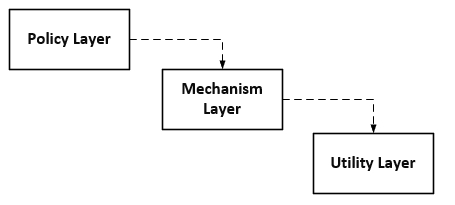
\includegraphics[width=10cm]{Naivelayeringscheme.jpg}

但我们不希望在设计软件的时候，上层依赖于下层的详细实现，避免因为下面的实现细节改动影响上层模块。
如果用UML的表示，下图是面向对象设计方式：

%\href{文件:Invertedlayering_1.jpg}{650px}

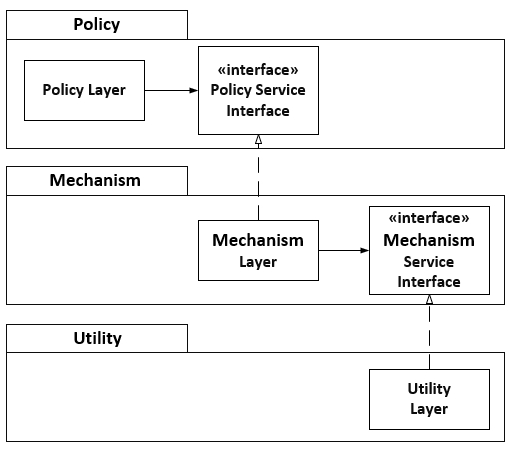
\includegraphics[width=10cm]{Invertedlayering_1.jpg}

上层只看到下面的接口，不会直接在代码里具体放某一个对象object，这样就可以避免下面详细的代码影响上层代码。上层可以利用接口调用到下层，但上层代码不会包含下层的具体对象(object)，这样就保持了灵活性。\\
实例说明：MVC（model view
controller）框架把显示、模型、控制（例如经键盘输入）分隔开，大部分应用系统会用不同的显示方式表达数据，例如饼状图、柱状图等。

\href{文件:Lean2.jpg}{650px}

%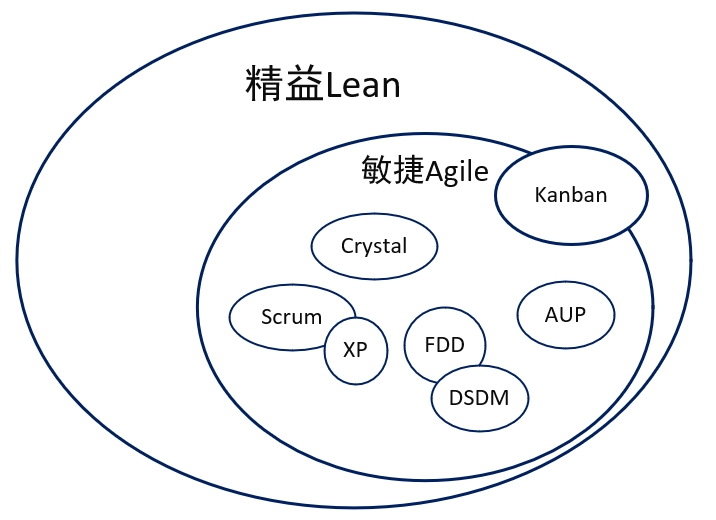
\includegraphics[width=10cm]{Lean2.jpg}

按MVC框架，使用view里的模块做展示，里面包括各种图形展示方式或报表方式，但view跟模型数据模块是隔开的，双互独立。若要新增柱状图方式展示数据，只需要在view里增加支持柱状图展示的代码便可，其他模块不受影响。\\
同样思路也可以用于controller，我们不仅需要展示，可能需要接收不同的输入方式，例如传统键盘，但如果后面需要使用弹出模拟键盘，也可以只增加模拟键盘的代码，但controller主程序不受影响。\\
细节方面里面view跟controller的体现方式会有区分。view通常可能会有多层展示，例如报表可能只使用饼状图，但有些报表可能要包含饼状图、柱状图、和表格等合成。但如果是刚才controller，就只有某一种方式，不会拼起来用的。\\
前者是一种设计模式，叫组合(Composite)模式。也满足开闭原则 (Open Closed
Principle OCP)软件应对变更关闭；对扩展开放。

%\href{文件:tdd_3-1.jpg}{650px}

\includegraphics[width=10cm]{tdd_3-1.jpg}

aComposite也可以包含另一个aComposite，做成多层组合 (nested Composite)

%\href{文件:tdd_3-2.jpg}{650px}

\includegraphics[width=10cm]{tdd_3-2.jpg}

后者叫策划(Strategy)模式。也满足依赖反转原则 (Dependency Inversion
Principle
DIP)：上层模块不应依赖于下层模块；都应依赖于抽象；细节应依赖于抽象，应针对接口编程，不针对实现。

%\href{文件:tdd_1.jpg}{650px}

\includegraphics[width=10cm]{tdd_1.jpg}

所以重构不仅仅写好变量名称，减少代码拷贝粘贴，更应包括如何管理模块之间的依赖关系、耦合度等。\\
当我们做重构时，应考虑这些原则和设计模式，有点像乐高积木一样，帮我们系统地设计软件。\\
希望任何功能的改变，尽量不会影响上层的代码，让整个系统更灵活，保持总体架构容易维护，更要让其他人能理解、读懂。\\
所以，如果了解面向对象的原理，再配上定期重构，就可以避免出现死代码。这是长期学习过程，除了培训和自学，也可以利用评审促进。例如让经验丰富的组长检查代码与设计，让经验少的编码人员尽早知道问题所在并改善。\\
``我很忙，哪有空做这些计划并记录？''\\
做这些记录，每天绝对不会占用超过15分钟时间，但好比锻炼马拉松，有度量才能知道今天跑一公里多少分钟，有没有进步或保持。我首次感到这习惯受用是十多年前考CMMI培训师，观察员（考官）会记录我每个模块实际花的时间，与计划对比。因为每天培训时间有限，必须在计划时间内完成。我一直保留这习惯：每天培训前，先在本子上写上计划时间，培训过程里记录实际时间，每天培训结束后在XLS里把计划与实际都记录。好处：我下次再培训同样内容就能更好策划实际的分配，也提醒我每个模块不能超时。
这方法能适用于任何活动，帮助估算：例如，我发现常常低估一些编程和写分享文章的工作量（因少做，不熟悉），但一些重复性工作会越来越快。这方法也能帮助避免无限拖延。所以回报能远远超越投入的工时。\\
如果团队有每次迭代冲刺回顾，以上的个人数据可归纳为团队数据，团队所有成员一起分析，制定下轮的改进措施。当然，采用相应的工具和技术，可以更好的提高效率，多记录，少占用时间。

\hypertarget{ux8f6fux4ef6ux5f00ux53d1ux4ee5ux5916}{%
\subsubsection{软件开发以外}\label{ux8f6fux4ef6ux5f00ux53d1ux4ee5ux5916}}

能让读者继续读下去的书，必须有头有尾，前后贯穿，有节奏。当我准备这一版时，就发现前面的版本都只是原始资料，没有组织好，除了要调整架构提高可读性外，还有很多多余的文字，须要精简。\\
代码重构也是同样的过程。只是勉强写好通过测试，程序员应该像工匠一样，精益求精，最后写出大家能容易读懂的代码，并经得起时间考验，方便维护。\\
书写得不好，读者可以选择不继续读下去，但程序没有写好，后果可能致命，所以管理者应关注代码的质量，不要以为程序通过测试，能按时交付，就算完事，只是开始。

\textbf{本章最佳实践对应}：

\begin{itemize}
\tightlist
\item
  CMMI

  \begin{itemize}
  \tightlist
  \item
    单元测试：PI 2.4 , OO设计：TS 2.1
  \end{itemize}
\item
  XP

  \begin{itemize}
  \tightlist
  \item
    测试驱动开发TDD、重构、编码标准都是XP里的实践
  \end{itemize}
\end{itemize}

\hypertarget{ux53c2ux8003-references}{%
\section{参考 References}\label{ux53c2ux8003-references}}

\begin{enumerate}
\tightlist
\item
  Gamma, Erich , \emph{Design Patterns: Elements of Reusable
  Object-Oriented Software} (1997) Addison Wesley\\
\item
  Fowler, M., \emph{Refactoring}2/e (2019) Pearson Education\\
\item
  Martin, Robert C, \emph{Agile Software Development: Principles,
  Patterns, and Practices} (2002) Prentice Hall\\
\end{enumerate}




